\documentclass[11pt, twocolumn]{article}

\usepackage[spanish]{babel}
\usepackage[none]{hyphenat}
\usepackage[left=1.5cm, right=1.5cm, top = 2cm, bottom=2.5cm]{geometry}
\usepackage{parskip}
\usepackage[export]{adjustbox}
\usepackage{enumitem}
\usepackage{listings}
\usepackage{color}
\usepackage{fancyhdr}
\usepackage{graphicx}
\usepackage{caption}
% \usepackage{subcaption}
% \usepackage{wrapfig}
% \usepackage{longtable}
% \usepackage{multirow, makecell}
% \usepackage{amsmath} 
\usepackage{amsfonts}
\usepackage[hidelinks]{hyperref}
\usepackage{csquotes}

\newcommand{\linejump}{\hfill \break}
\renewcommand{\thefootnote}{\fnsymbol{footnote}}
% \newcommand{\unit}[1]{\ensuremath{\, \mathrm{#1}}}

\definecolor{dkgreen}{rgb}{0,0.6,0}
\definecolor{gray}{rgb}{0.5,0.5,0.5}
\definecolor{mauve}{rgb}{0.58,0,0.82}
\lstset{
  language=Java,
  aboveskip=3mm,
  belowskip=3mm,
  showstringspaces=false,
  columns=flexible,
  basicstyle={\tiny\ttfamily},
  numbers=none,
  numberstyle=\tiny\color{gray},
  keywordstyle=\color{blue},
  commentstyle=\color{dkgreen},
  stringstyle=\color{mauve},
  breaklines=true,
  breakatwhitespace=true,
  tabsize=2
}

\sloppy
\setlength{\parindent}{0cm}
\setlength{\columnsep}{0.5cm}
\decimalpoint
\graphicspath{{img/}}

\hypersetup{colorlinks=true, urlcolor=blue, citecolor=blue}
\urlstyle{same}

\pagestyle{fancyplain}
\fancyhf{}
\fancyhead[L]{\scriptsize 
  Universidad Nacional Autónoma de México \\
  Laboratorio de Programación Orientada a Objetos \\
  M.C. Leonardo Ledesma Dominguez
}
\fancyhead[R]{\thepage}


\begin{document}
  \twocolumn[
    \centering
    Acosta Porcayo Alan Omar, Gutiérrez Grimaldo Alejandro, Medina Villa Samuel

    \linejump

    \LARGE \textbf{Práctica 7. Herencia} \\
    
    \linejump
  ]
      
  \footnotetext{
    \scriptsize 
    Acosta Porcayo Alan Omar Ing. en Computación 320206102 \\
    Gutiérrez Grimaldo Alejandro Ing. en Computación 320282098 \\
    Medina Villa Samuel Ing. en Computación 320249538
  }
        
  \fancyfoot{}

  \section*{Resumen}
  El objetivo es implementar los conceptos de herencia en un lenguaje de programación orientado a objetos, lo que implica crear clases que se basan en otras, estableciendo una jerarquía de clases. En esencia, se busca aprovechar la capacidad de una clase secundaria para heredar propiedades y métodos de una clase principal, lo que permite una organización y reutilización eficiente del código en un programa orientado a objetos.

  \section*{Introducción}
  La herencia es omnipresente en la programación orientada a objetos, ya que permite que las clases hereden propiedades y métodos de otras clases. Esto fomenta la reutilización de código y facilita la organización de un programa.

  \subsection*{Jerarquía de Clases}
  En la herencia, se establece una jerarquía de clases, con una ``superclase'' o ``clase base'' que se utiliza como base para crear ``subclases'' o ``clases derivadas''. Las clases derivadas heredan todas las propiedades y métodos de la clase base y pueden agregar los suyos propios.

  \subsection*{Relación \textit{IS-A} y \textit{HAS-A}}
  En la herencia, se establece la relación \textit{``IS-A''}, lo que significa que una clase derivada es un tipo específico de la clase base. También se menciona la relación \textit{``HAS-A''}, que se basa en la composición y se refiere a la inclusión de una referencia de una clase en otra.

  \subsection*{Clase \textit{Object}}
  En lenguajes de programación orientados a objetos como Java, todas las clases heredan implícitamente de la clase \textit{Object}. Esto significa que todas las clases poseen métodos como \textit{clone, equals, hashCode, notify} y otros definidos en \textit{Object}.

  \subsection*{Sobrescritura (\textit{Overriding})}
  La sobrescritura se refiere a la capacidad de una subclase para redefinir el comportamiento de un método heredado de la clase base. Esto permite ajustar el comportamiento de un método de acuerdo con las necesidades de cada clase.

  \subsection*{Constructores en la Herencia}
  Los constructores son métodos especiales utilizados para inicializar los atributos de un objeto. Cuando se crea un objeto de una clase derivada, se crea implícitamente un objeto de la clase base con su constructor correspondiente. Se explica cómo se pueden invocar constructores sobrecargados y acceder a elementos de la clase base utilizando la palabra reservada ``super''.

  \subsection*{Sobrecarga (\textit{Overloading}) vs. Sobrescritura (\textit{Overriding})}
  Se destacan las diferencias entre la sobrecarga y la sobrescritura. La sobrecarga implica definir varios métodos con el mismo nombre en una clase, pero con diferentes tipos y números de parámetros, mientras que la sobrescritura se aplica a la herencia y permite redefinir métodos heredados en subclases.

  \section*{Objetivos}
  \begin{itemize}
    \item Crear una estructura de clases que muestre una relación jerárquica sólida, con una clase base y múltiples clases derivadas, para demostrar cómo la herencia puede facilitar la organización del código.
    \item Utilizar la herencia para reutilizar propiedades y métodos de la clase base en las clases derivadas, mostrando cómo esta técnica simplifica el desarrollo al evitar la duplicación de código.
    \item Implementar los conceptos de herencia en un lenguaje de programación orientado a objetos.
  \end{itemize}

  \section*{Metodología} 
  \subsection*{Ejercicio realizado por el profesor}
  Ejemplo de herencia
  \textbf{Clase \textit{Vehiculo}} 
  \begin{lstlisting}
package practica7;

public class Vehiculo {
  private String numSerie = "";

  public String getNumSerie() {
    return numSerie;
  }

  public void setNumSerie(String a) {
    this.numSerie = a;
  }

  @Override
  public String toString() {
    return "Vehiculo{" + "numSerie=" + numSerie + '}';
  }
}
  \end{lstlisting}

  \textbf{Clase \textit{Automovil}}
  \begin{lstlisting}
package practica7;

public class Automovil extends Vehiculo {
  public Automovil() {
    super();
  }
}
  \end{lstlisting}

  \textbf{Clase \textit{AutoElectrico}}
  \begin{lstlisting}
package practica7;

public class AutoElectrico extends Automovil{
    
}
  \end{lstlisting}

  \textbf{Clase \textit{Avion}}
  \begin{lstlisting}
package practica7;

public class Avion extends Vehiculo{
      
}
  \end{lstlisting}

  \textbf{Clase \textit{Barco}}
  \begin{lstlisting}
package practica7;

public class Barco extends Vehiculo {
  @Override
  public String toString() {
    //System.out.println(super.toString());
    return "Barco{" + "numSerie=" + getNumSerie() + '}';
  }
}
  \end{lstlisting}

  \textbf{Clase \textit{Fabrica}}
  \begin{lstlisting}
package practica7;

public class Fabrica {
  public static void main(String[] args) {
    Vehiculo a = new Avion(); //Upcasting
    
    if (a instanceof Avion) {
      System.out.println("a es una instancia de Avion");
    }
    if (a instanceof Vehiculo) {
      System.out.println("a es una instancia de Vehiculo");
    }
    //Avion b = new Vehiculo();

    Vehiculo b = (Vehiculo) a;
    if (b instanceof Avion) {
      System.out.println("b es una instancia de Avion");
    }
    if (b instanceof Vehiculo) {
      System.out.println("b es una instancia de Vehiculo");
    }

    Barco titanic = new Barco();
    titanic.setNumSerie("KLA0009101");
    System.out.println(titanic);

    Automovil mercedes = new Automovil();
    mercedes.setNumSerie("MNX0009101");
    System.out.println(mercedes);

    Avion boeing = new Avion();
    boeing.setNumSerie("BOE0009101");
    System.out.println(boeing);
  }
}
  \end{lstlisting}

  \section*{Resultados}
  \subsection*{Problema 1}
  Investigue el uso de \textit{ENUM} y aplíquelo en el ejemplo visto en laboratorio para:
  \begin{enumerate}[label=\alph*.]
    \item Crear tipos de aviones supersónicos, militares, turísticos y de carga.
    \item Escriba en sus conclusiones de este reporte, a qué se parece la estructura \textit{ENUM}.
  \end{enumerate}

  \linejump
  \textbf{Clase \textit{Vehiculo}}
  \begin{lstlisting}
package practica7.ejercicio1;

public class Vehiculo {
  private String numSerie = "";

  public String getNumSerie() {
    return numSerie;
  }

  public void setNumSerie(String a) {
    this.numSerie = a;
  }

  @Override

  public String toString() {
    return "Vehiculo{" + "numSerie=" + numSerie + '}';
  }
}
  \end{lstlisting}

  \textbf{Clase \textit{Automovil}}
  \begin{lstlisting}
package practica7.ejercicio1;

public class Automovil extends Vehiculo {
  public Automovil() {
    super();
  }
}
  \end{lstlisting}

  \textbf{Clase \textit{AutoElectrico}}
  \begin{lstlisting}
  package practica7.ejercicio1;

  public class AutoElectrico extends Automovil{
      
  }
  \end{lstlisting}

  \textbf{Clase \textit{Avion}}
  \begin{lstlisting}
package practica7.ejercicio1;

public class Avion extends Vehiculo{
  //enum some differents kinds of airplanes
  public enum TipoAvion {
    supersonico, militar, turustico, carga
  }

  private TipoAvion tipo;

  public Avion(TipoAvion tipo) {
    this.tipo = tipo;
  }

  public TipoAvion getTipo() {
    return tipo;
  }

  public void setTipo(TipoAvion tipo) {
    this.tipo = tipo;
  } 
}
  \end{lstlisting}

  \textbf{Clase \textit{Barco}}
  \begin{lstlisting}
package practica7.ejercicio1;

public class Barco extends Vehiculo {
  @Override
  public String toString() {
    //System.out.println(super.toString());
    return "Barco{" + "numSerie=" + getNumSerie() + '}';
  }
}
  \end{lstlisting}

  \textbf{Clase \textit{Fabrica}}
  \begin{lstlisting}
package practica7.ejercicio1;

public class Fabrica {
  public static void main(String[] args) {
      
    //Avion supersonico
    Avion caza = new Avion(Avion.TipoAvion.supersonico);
    caza.setNumSerie("CAZ0009101");
    System.out.println(caza);
    if (caza instanceof Avion) {
      System.out.println("caza es una instancia de Avion");
    }
    if (caza instanceof Vehiculo) {
      System.out.println("caza es una instancia de Vehiculo");
    }

    // Avion militar
    Avion concorde = new Avion(Avion.TipoAvion.militar);
    concorde.setNumSerie("CON0009101");
    System.out.println(concorde);
    if (concorde instanceof Avion) {
      System.out.println("concorde es una instancia de Avion");
    }
    if (concorde instanceof Vehiculo) {
      System.out.println("concorde es una instancia de Vehiculo");
    }

    // Avion turistico
    Avion boeing = new Avion(Avion.TipoAvion.turustico);
    boeing.setNumSerie("BOE0009101");
    System.out.println(boeing);
    if (boeing instanceof Avion) {
      System.out.println("boeing es una instancia de Avion");
    }
    if (boeing instanceof Vehiculo) {
      System.out.println("boeing es una instancia de Vehiculo");
    }

    //Avion de carga
    Avion airbus = new Avion(Avion.TipoAvion.carga);
    airbus.setNumSerie("AIR0009101");
    System.out.println(airbus);
    if (airbus instanceof Avion) {
      System.out.println("airbus es una instancia de Avion");
    }
    if (airbus instanceof Vehiculo) {
      System.out.println("airbus es una instancia de Vehiculo");
    }   
  }
}
  \end{lstlisting}
  
  \textbf{Ejecución}
  \begin{figure}[ht]
    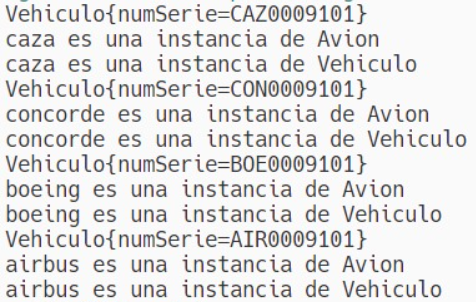
\includegraphics[width=0.6\columnwidth, center]{P1.png}
  \end{figure}

  \subsection*{Problema 2}
  Utilice el código visto en laboratorio para crear una competencia de carreras, considere:
  \begin{enumerate}[label=\alph*.]
    \item La variable velocidad inicial de tipo privada para cada objeto creado.
    \item Una variable de aceleración/desaceleración que se determine como un numero
    aleatorio entre 1-20 ($+/-$ 10)
    \item Realice una simulación de carreras entre tipos de \textit{Vehículo} en una pista de
    longitud de 1000 km, utilice un ciclo \textit{for} para simular el tiempo $t$. Calcule la
    distancia recorrida usando la velocidad inicial y decrementando o incrementando
    la aceleración del número aleatorio (que será distinta para cada vehículo y para
    cada instante $t$).
    \item Cree usando \textit{HASH TABLE} que contenga al menos un vehículo por cada tipo.
    \item Coloque en consola la sig. Salida (Ejemplo):
  \end{enumerate}

  \newpage
  \begin{figure}[ht]
    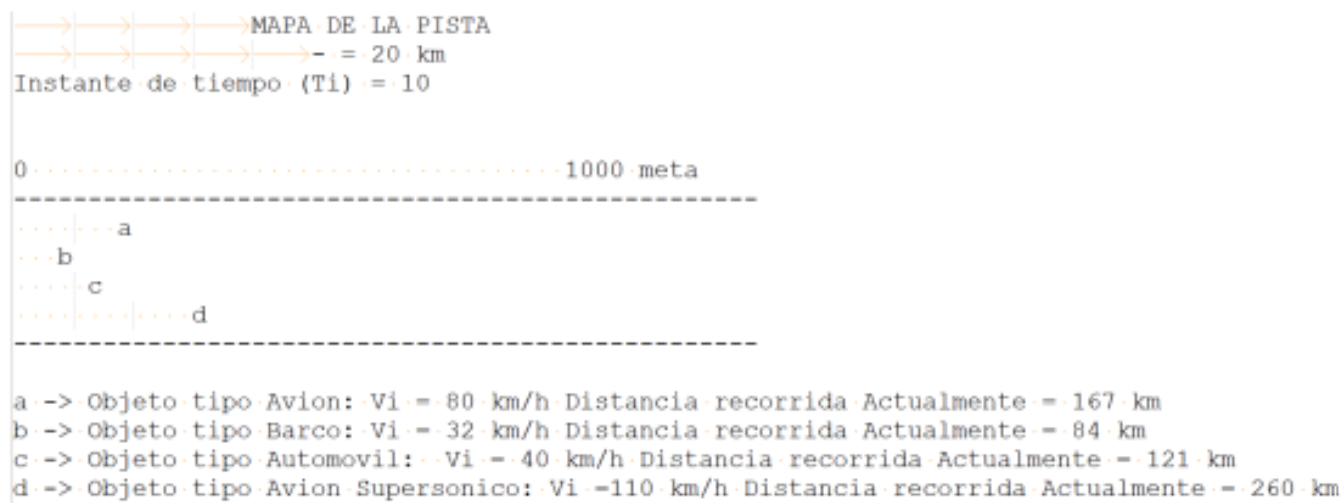
\includegraphics[width=\columnwidth, center]{pista.png}
  \end{figure}

  \linejump
  \textbf{Clase \textit{Vehiculo}}
  \begin{lstlisting}
package practica7.ejercicio2;

import java.util.Random;

public class Vehiculo {
  private String numSerie = "";
  private int velocidadInicial;
  private int aceleracionDesaceleracion;

  public String getNumSerie() {
    return numSerie;
  }

  public void setNumSerie(String a) {
    this.numSerie = a;
  }

  public Vehiculo() {
    Random rand = new Random();
    velocidadInicial = rand.nextInt(100) + 1;
    aceleracionDesaceleracion = rand.nextInt(20) - 10;
  }

  public int getVelocidadInicial() {
    return velocidadInicial;
  }

  public int getAceleracionDesaceleracion() {
    return aceleracionDesaceleracion;
  }

  @Override
  public String toString() {
      return "Vehiculo{" + "numSerie=" + numSerie + '}';
  }
}
  \end{lstlisting}
  
  \textbf{Clase \textit{Automovil}}
  \begin{lstlisting}
package practica7.ejercicio2;

public class Automovil extends Vehiculo {
  public Automovil() {
    super();
  }
}
  \end{lstlisting}

  \textbf{Clase \textit{AutoElectrico}}
  \begin{lstlisting}
package practica7.ejercicio2;

import java.util.Random;

public class AutoElectrico extends Automovil {
  private int velocidadInicial;
  private int aceleracionDesaceleracion;

  public AutoElectrico() {
    Random rand = new Random();
    velocidadInicial = rand.nextInt(100) + 1;
    aceleracionDesaceleracion = rand.nextInt(20) - 10;
  }

  public int getVelocidadInicial() {
    return velocidadInicial;
  }

  public int getAceleracionDesaceleracion() {
    return aceleracionDesaceleracion;
  }
}
  \end{lstlisting}

  \textbf{Clase \textit{Avion}}
  \begin{lstlisting}
package practica7.ejercicio2;

import java.util.Random;

public class Avion extends Vehiculo {
  private int velocidadInicial;
  private int aceleracionDesaceleracion;

  public Avion() {
    Random rand = new Random();
    velocidadInicial = rand.nextInt(100) + 1;
    aceleracionDesaceleracion = rand.nextInt(20) - 10;
  }

  public int getVelocidadInicial() {
    return velocidadInicial;
  }

  public int getAceleracionDesaceleracion() {
    return aceleracionDesaceleracion;
  }
}
  \end{lstlisting}

  \textbf{Clase \textit{AvionSupersonico}}
  \begin{lstlisting}
package practica7.ejercicio2;

import java.util.Random;

class AvionSupersonico extends Avion{
  private int velocidadInicial;
  private int aceleracionDesaceleracion;

  public AvionSupersonico() {
    Random rand = new Random();
    velocidadInicial = rand.nextInt(100) + 1;
    aceleracionDesaceleracion = rand.nextInt(20) - 10;
  }

  public int getVelocidadInicial() {
    return velocidadInicial;
  }

  public int getAceleracionDesaceleracion() {
    return aceleracionDesaceleracion;
  }
}
  \end{lstlisting}

  \textbf{Clase \textit{Barco}}
  \begin{lstlisting}
package practica7.ejercicio2;

import java.util.Random;

public class Barco extends Vehiculo {
  private int velocidadInicial;
  private int aceleracionDesaceleracion;

  public Barco() {
    Random rand = new Random();
    velocidadInicial = rand.nextInt(100) + 1;
    aceleracionDesaceleracion = rand.nextInt(20) - 10;
  }

  public int getVelocidadInicial() {
    return velocidadInicial;
  }

  public int getAceleracionDesaceleracion() {
    return aceleracionDesaceleracion;
  }
}
  \end{lstlisting}

  \textbf{Clase \textit{Fabrica}}
  \begin{lstlisting}
package practica7.ejercicio2;

import java.util.Hashtable;

public class Fabrica {
  public static void main(String[] args) {
    Avion avion = new Avion();
    Barco barco = new Barco();
    AvionSupersonico avionSupersonico = new AvionSupersonico();
    Automovil automovil = new Automovil();

    Vehiculo[] vehiculos = { avion, barco, avionSupersonico, automovil };

    Hashtable<String, Vehiculo> vehiculosHash = new Hashtable<>();

    vehiculosHash.put(avion.getNumSerie(), avion);
    vehiculosHash.put(barco.getNumSerie(), barco);
    vehiculosHash.put(avionSupersonico.getNumSerie(), avionSupersonico);
    vehiculosHash.put(automovil.getNumSerie(), automovil);

    int longitudPista = 20;
    Vehiculo ganador = null;
    int tiempoGanador = Integer.MAX_VALUE;

    int tiempo = 0;

    while (ganador == null) {
      System.out.printf("MAPA DE LA PISTA");
      System.out.println("Instante de tiempo: " + tiempo + " min");
      System.out.println("0.............20 meta");
      System.out.println("-------------------------");
      boolean todosLlegaron = true;
      for (int i = 0; i < vehiculos.length; i++) {
        Vehiculo vehiculo = vehiculos[i];

        int aceleracionAleatoria = vehiculo.getAceleracionDesaceleracion(); 
        int nuevaVelocidad = vehiculo.getVelocidadInicial() + aceleracionAleatoria;

        if (nuevaVelocidad < 0) {
          nuevaVelocidad = 0;
        }

        int distanciaRecorrida = (nuevaVelocidad * tiempo) / 60; 

        if (distanciaRecorrida < longitudPista) {
          todosLlegaron = false;
        }

        StringBuilder pista = new StringBuilder("....................");
        char etiqueta = (char) ('a' + i);
        pista.setCharAt(distanciaRecorrida >= 19 ? 19 : distanciaRecorrida, etiqueta);

        String nombreVehiculo = vehiculo.getClass().getSimpleName();
        String distanciaRecorridaStr = String.valueOf(distanciaRecorrida);
        String velocidadStr = String.valueOf(nuevaVelocidad);
        System.out.printf("%s\n", pista);
        System.out.printf("%c -> Objeto tipo %s: Vi = %s km/h 
                Distancia recorrida Actualmente = %s km\n",
                etiqueta, nombreVehiculo, velocidadStr, distanciaRecorridaStr);

        if (distanciaRecorrida >= longitudPista) {
          if (tiempo < tiempoGanador) {
            ganador = vehiculo;
            tiempoGanador = tiempo;
          }
        }
      }

      if (todosLlegaron) {
        break; 
      }

      tiempo += 1; 
      try {
        Thread.sleep(1000); 
      } catch (InterruptedException e) {
        e.printStackTrace();
      }
      System.out.print("\033[H\033[2J");
      System.out.flush();
    }

    System.out.println("-------------------------");
    if (ganador != null) {
      System.out.println("El ganador es: " + ganador.getClass().getSimpleName());
      System.out.println("Tiempo del ganador: " + tiempoGanador + " min");
    }
  }
}
  \end{lstlisting}  
  
  \newpage
  \textbf{Ejecución}
  \begin{figure}[ht]
    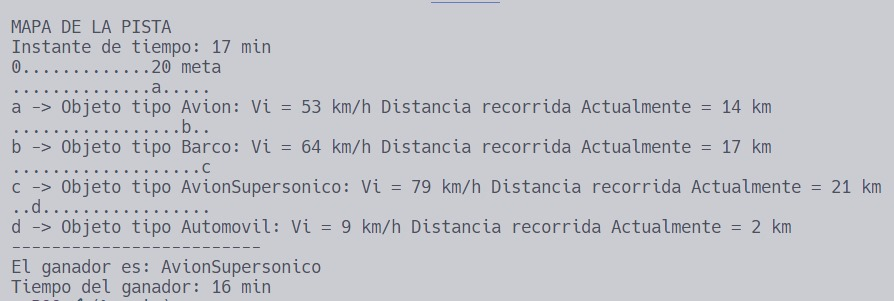
\includegraphics[width=\columnwidth, center]{P2.jpg}
  \end{figure}

  \subsection*{Problema 3}
  Implemente la estructura de los conjuntos numerales que usamos en Matemáticas. Siguiendo la siguiente jerarquía:
  \begin{figure}[ht]
    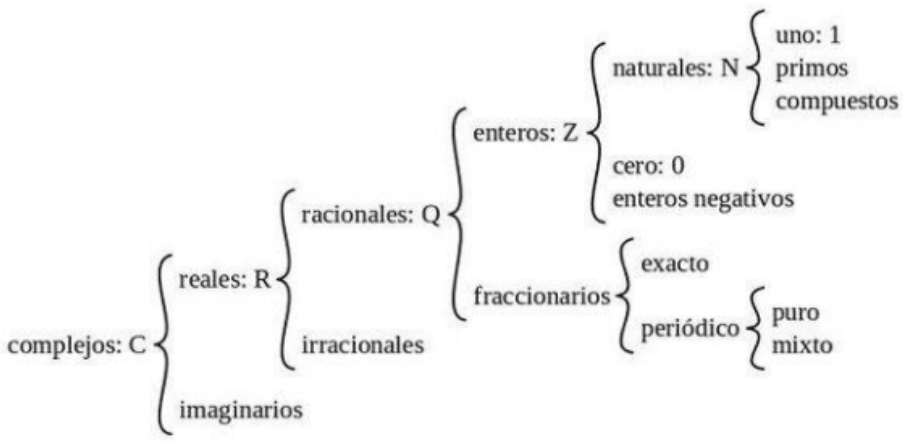
\includegraphics[width=\columnwidth, center]{jerarquia.png}
  \end{figure}

  Donde se aplique la herencia considerando las atributos y métodos que considere, por ejemplo, considere el atributo de conmutatividad y cerradura y un método existencia de elemento idéntico y obtenga ese elemento. Aplique propiedades propias del polimorfismo dinámico y estático, así como super.
  
  Tome en cuenta lo siguiente:
  \begin{itemize}
    \item $\mathbb{I}$ los números imaginarios se deben modelar con una clase de tipo \textit{final}, dado que ya no puede heredar.
    \item No considere a los números fraccionarios ni sus divisiones, entiéndase que son
    racionales.
    \item No considere las divisiones de lo naturales, solo manéjelos como conjunto general.
    \item Considere al 0 como una clase final.
  \end{itemize}

  \linejump  
  \textbf{Clase \textit{Complejos}}
  \begin{lstlisting}
public class Complejos {
  private double parteReal;
  private double parteImaginaria;

  public Complejos() {}

  public Complejos(double parteReal, double parteImaginaria) {
    this.parteReal = parteReal;
    this.parteImaginaria = parteImaginaria;
  }

  public double getParteReal() {
    return parteReal;
  }

  public void setParteReal(double parteReal) {
    this.parteReal = parteReal;
  }

  public double getParteImaginaria() {
    return parteImaginaria;
  }

  public void setParteImaginaria(double parteImaginaria) {
    this.parteImaginaria = parteImaginaria;
  }

  public boolean pertenece() {
    return this instanceof Complejos;
  }

  public String elementoIdentico() {
    return "0.0";
  }

  public String inversoAditivo() {
    return "(" + (-parteReal) + ", " + (-parteImaginaria) + ")";
  }

  public String inversoMultiplicativo() {
    return "(" + (parteReal / 
    (parteReal * parteReal + parteImaginaria * parteImaginaria)) 
    + ", " + 
    (-parteImaginaria / 
    (parteReal * parteReal + parteImaginaria * parteImaginaria)) + ")";
  }


  public String toString() {
    return "Complejos";
  }
}  
  \end{lstlisting}

  \textbf{Clase \textit{Reales}}
  \begin{lstlisting}
public class Reales extends Complejos {
  private double valor;

  public Reales() {
    super();
  }

  public Reales(double valor) {
    super();
    this.valor = valor;
  }

  public double getValor() {
    return valor;
  }

  public void setValor(double valor) {
    this.valor = valor;
  }

  @Override
  public boolean pertenece() {
    return this instanceof Reales;
  }

  @Override
  public String elementoIdentico() {
    return "0.0";
  }

  @Override
  public String inversoAditivo() {
    return "" + (-valor);
  }

  @Override
  public String inversoMultiplicativo() {
    return "" + (1 / valor);
  }

  @Override
  public String toString() {
    return "Reales";
  }
}
  \end{lstlisting}

  \textbf{Clase \textit{Imaginarios}}
  \begin{lstlisting}
public final class Imaginarios extends Complejos{
  private double parteReal;
  private double parteImaginaria;

  public Imaginarios() {
    super();
  }

  public Imaginarios(double parteReal, double parteImaginaria) {
    super();
    this.parteReal = parteReal;
    this.parteImaginaria = parteImaginaria;
  }

  public double getParteReal() {
    return parteReal;
  }

  public void setParteReal(double parteReal) {
    this.parteReal = parteReal;
  }

  public double getParteImaginaria() {
    return parteImaginaria;
  }

  public void setParteImaginaria(double parteImaginaria) {
    this.parteImaginaria = parteImaginaria;
  }

  @Override
  public boolean pertenece() {
    return this instanceof Imaginarios;
  }

  @Override
  public String elementoIdentico() {
    return "0.0";
  }

  @Override
  public String inversoAditivo() {
    return "(" + (-parteReal) + ", " + (-parteImaginaria) + ")";
  }

  @Override
  public String inversoMultiplicativo() {
    return "(" + (parteReal / 
    (parteReal * parteReal + parteImaginaria * parteImaginaria)) 
    + ", " + 
    (-parteImaginaria / 
    (parteReal * parteReal + parteImaginaria * parteImaginaria)) + ")";
  }

  @Override
  public String toString() {
    return "Imaginarios";
  }
}  
  \end{lstlisting}

  \textbf{Clase \textit{Racionales}}
  \begin{lstlisting}
public class Racionales extends Reales{
  private double valor;

  public Racionales(){
    super();
  }

  public Racionales(double valor){
    super();
    this.valor = valor;
  }

  public double getValor(){
    return valor;
  }

  public void setValor(double valor){
    this.valor = valor;
  }
  
  @Override
  public boolean pertenece(){
    return this instanceof Racionales;
  }

  @Override
  public String elementoIdentico(){
    return "0.0";
  }

  @Override
  public String inversoAditivo(){
    return "" + (-valor);
  }

  @Override
  public String inversoMultiplicativo(){
    return "" + (1/valor);
  }
  
  @Override
  public String toString(){
    return "Racionales";
  }
}
  \end{lstlisting}

  \textbf{Clase \textit{Irracionales}}
  \begin{lstlisting}
public final class Irracionales extends Reales{
  private double valor;

  public Irracionales(){
    super();
  }

  public Irracionales(double valor){
    super();
    this.valor = valor;
  }

  public double getValor(){
    return valor;
  }

  public void setValor(double valor){
    this.valor = valor;
  }

  @Override
  public boolean pertenece(){
    return this instanceof Irracionales;
  }

  @Override
  public String elementoIdentico(){
    return "No existe elemento identico";
  }

  @Override
  public String inversoAditivo(){
    return "No existe inverso aditivo";
  }

  @Override
  public String inversoMultiplicativo(){
    return "No existe inverso multiplicativo";
  }

  @Override
  public String toString(){
    return "Irracionales";
  }
}  
  \end{lstlisting}
  
  \textbf{Clase \textit{Enteros}}
  \begin{lstlisting}
public class Enteros extends Racionales {
  private int valor;

  public Enteros(){
    super();
  }
  
  public Enteros(int valor){
    super();
    this.valor = valor;
  }

  public int getValorE(){
    return valor;
  }

  public void setValorE(int valor){
    this.valor = valor;
  }

  @Override
  public boolean pertenece(){
    return this instanceof Enteros;
  }

  @Override
  public String elementoIdentico(){
    return "0";
  }

  @Override
  public String inversoAditivo(){
    return "" + (-valor);
  }

  @Override
  public String inversoMultiplicativo(){
    return (this.valor == 1) ? "1" : "No existe inverso multiplicativo";
  }
  
  @Override
  public String toString(){
    return "Enteros";
  }
}  
  \end{lstlisting}

  \textbf{Clase \textit{Naturales}}
  \begin{lstlisting}
public class Naturales extends Enteros {
  private int valor;

  public Naturales() {
    super();
  }

  public Naturales(int valor) {
    super();
    this.valor = valor;
  }

  public int getValorN() {
    return valor;
  }

  public void setValorN(int valor) {
    this.valor = valor;
  }

  @Override
  public boolean pertenece() {
    return this instanceof Naturales;
  }

  @Override
  public String elementoIdentico() {
    return "1";
  }

  @Override
  public String inversoAditivo() {
    return "No existe inverso aditivo";
  }

  @Override
  public String inversoMultiplicativo() {
    return (this.valor == 1) ? "1" : "No existe inverso multiplicativo";
  }

  @Override
  public String toString() {
    return "Naturales";
  }    
}  
  \end{lstlisting}

  \textbf{Clase \textit{Cero}}
  \begin{lstlisting}
public final class Cero extends Enteros {
  final int valor = 0;

  public Cero() {
    super();
  }

  public int getValorC() {
    return valor;
  }

  @Override
  public boolean pertenece() {
    return this instanceof Cero;
  }

  @Override
  public String elementoIdentico() {
    return "0";
  }

  @Override
  public String inversoAditivo() {
    return "0";
  }

  @Override
  public String inversoMultiplicativo() {
    return "No existe inverso multiplicativo";
  }

  @Override
  public String toString() {
    return "Cero";
  }    
}  
  \end{lstlisting}

  \textbf{Clase \textit{EnterosNegativos}}
  \begin{lstlisting}
public class EnterosNegativos extends Enteros{
  private int valor;

  public EnterosNegativos(){
    super();
  }

  public EnterosNegativos(int valor){
    super();
    this.valor = valor;
  }

  public int getValorEN(){
    return valor;
  }

  public void setValorEN(int valor){
    this.valor = valor;
  }
  
  @Override
  public boolean pertenece(){
    return this instanceof EnterosNegativos;
  }

  @Override
  public String elementoIdentico(){
    return "0";
  }

  @Override
  public String inversoAditivo(){
    return "" + (-valor);
  }

  @Override
  public String inversoMultiplicativo(){
    return (this.valor == -1) ? "-1" : "No existe inverso multiplicativo";
  }

  @Override
  public String toString(){
    return "EnterosNegativos";
  }    
}  
  \end{lstlisting}

  \section*{Conclusiones}
  En resumen, la herencia en el contexto de la Programación Orientada a Objetos (POO) es un principio fundamental que posibilita la formación de una estructura jerárquica de clases, permitiendo que las clases derivadas hereden tanto propiedades como métodos de una clase base. 
  
  Esta característica de reutilización de código facilita la organización y la estructuración del software, lo que a su vez mejora la eficiencia en el proceso de desarrollo y en el mantenimiento del sistema. Además, la herencia capacita para modelar relaciones \textit{``IS-A''}, donde una subclase se considera un tipo específico de su superclase, reflejando de esta manera las relaciones entre objetos en el mundo real. 
  
  En última instancia, la herencia se erige como una herramienta poderosa que contribuye a la construcción de software más modular, expansible y de comprensión sencilla.

  \section*{Referencias}
  \small
  Solano, J. (2017, 20 enero). \textit{Manual de prácticas de Programación Orientada a Objetos}. Laboratorio de Computación Salas A y B. \url{http://lcp02.fi-b.unam.mx/} \\

  
\end{document}